To synchronize the video streams we use an synchronization technique presented in \cite{segundo2015remote}: the Remote Temporal Couplers for aligning videos. It allows us to synchronize independent videos from multiple sources and to infer unknown relations from videos. We implemented the technique under our Dynamic Alignment List structure.

A DAL derivates from a matrix m x n, with m and n natural numbers, where m=n is the quantity of videos that can be synchronized at that moment. Each position of the matrix represents the relation of two videos (the coupler), in other words, the value necessary to align them, in our synchronization scenario. This value is calculated using: $\Delta_{i,j}=begin(id_{i,0})-begin(id_{0,j}), para 0<i,j\neq m $, where begin(x) is the time where an asset X begins its presentation. A $\Delta_{i,j} > 0$, implies that the asset in the column starts $\Delta_{i,j}$ before the asset in the line. Case $\Delta_{i,j} < 0$, the opposite happens and case $Delta_{i,j} = 0$, both starts at the same time.

As previously said, the list is derived from a matrix, presenting different aspects. Firstly, it does not presents all cells of a matrix. In the matrix, $\Delta_{i,j}$ is equal to $\-Delta_{j,i}$, so we don't need to store both relations, and with that, only the superior part of the relations are stored. Secondly, each "cell" of the list, presents multiple properties to help in the management of the crowd contributions. As each relation can contain multiple contributions, we need to calculate a mean of these contributions  to set as the actual $\Delta$. Lastly, each relation has a new dimension: a list with all contributions for that relation, that identifies the value of the contribution and the user that made it (if we want to identify who made it).

Figure~\ref{dal}, shows the representation of a DAL. There we have 5 assets (videos in our scope) labelled: A, B, C, D and E. Each asset represents a struct with the assets: URI, label, duration and a list of relations with the other assets. Following the asset A we find its relations with the other assets: AB, AC, AD and AE. We do not need to represent AA because $\Delta_{A,A}$ is always 0. Taking teh relations from B, we have: BC, BD and BE.  Again, $\Delta_{B,B} = 0$. Thus, we do not represent BA, because we previously represented AB, and as said before, we can find BA by negating AB ($\Delta_{A,B} = -\Delta_{A,B}$). And this will happens to the other relations.

In the end of the DAL, we have the contributions for each asset (represented in the figure by a cloud due to figure dimensions). Each relation can receive multiple contributions, and are stored in the list. These contributions are processed (means) and generate the value of $\Delta$ for its relations. Fields such as confidence factor and number of contributions are used to know how robust those contributions are, and if its necessary more contributions to verify the synchronization.

\begin{figure}
	\centering
	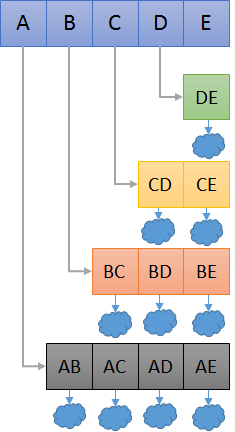
\includegraphics[scale=0.8]{figure/dal/dal}
	\caption{DAL with 5 Assets (A,B,C,D,E)}
	\label{dal}
\end{figure}

%%%%%%%%%%%%%%%%%%%%%%%%%% ACM %%%%%%%%%%%%%%%%%%

%Besides the synchronization method, there is the need to manage all the generated tasks: which pair of chunks will be sent to each user? From which videos? Where are the contributions stored? How can the contributions be validated? How to know that all videos are synchronized? What are the time offsets among the videos? Do I need to compare all videos?

%Trying to answer these questions, we developed the concept of a  Dynamic Alignment List. It is responsible for managing all contributions, checking the convergence of the contributions, distributing the videos, inferring unknown values and storing $\Delta$ values for each pair of videos.

%The DAL has two main features: (i) time offset and (ii) contribution managements. The time offset management deals with all videos relations manipulation while the contributions management takes care of the crowd management.



